\documentclass[a4paper]{article}
\usepackage[a4paper,margin=0mm]{geometry}
\usepackage{fontspec}
\usepackage{unicode-math}
\usepackage{tikz}
\usetikzlibrary{calc}
\usepackage[table]{xcolor}
\usepackage[absolute]{textpos}
\usepackage{enumitem}
\usepackage{array}
\usepackage{multirow}

\setmainfont{Libertinus Serif}
\setsansfont{Libertinus Sans}
\setmathfont{Libertinus Math}

\definecolor{accent}{HTML}{0F6A52}
\definecolor{badge}{HTML}{A9CFC2}
\definecolor{ink}{HTML}{2A2E30}

\setlength{\TPHorizModule}{1mm}
\setlength{\TPVertModule}{1mm}
\setlength{\parindent}{0pt}
\pagestyle{empty}
\binoppenalty=10000 \relpenalty=10000

\newcommand{\LCOL}{16mm}
\newcommand{\RCOL}{111mm}
\newcommand{\COLW}{83mm}

\newcommand{\topicheader}[2]{%
\begin{textblock*}{194mm}(16mm,10mm)
\begin{tikzpicture}
\node[fill=accent,text=white,font=\sffamily\bfseries\fontsize{13}{13}\selectfont,
      minimum width=9mm,minimum height=9mm,inner sep=0pt] at (4.5mm,-4.5mm) {#1};
\node[font=\sffamily\bfseries\fontsize{15}{16}\selectfont,text=ink,anchor=west] at (12mm,-4.5mm) {#2};
\end{tikzpicture}
\end{textblock*}
\begin{textblock*}{194mm}(16mm,22.5mm)

\begin{tikzpicture}
\fill[accent] (0,0) rectangle (194mm,0.5mm);
\end{tikzpicture}
\end{textblock*}
}

\newcommand{\pagefooter}[1]{%
\begin{textblock*}{194mm}(8mm,286.41mm)
  
\begin{tikzpicture}
    \fill[accent] (0,0) rectangle (194mm,0.6mm);
  \end{tikzpicture}
\end{textblock*}
\begin{textblock*}{63.59mm}(8mm,288.27mm)
  {\sffamily\bfseries\color{accent}\fontsize{13}{16}\selectfont SAT 1200+}
\end{textblock*}
\begin{textblock*}{10mm}(188mm,288.27mm)
  \centering{\sffamily\color{accent}\fontsize{14}{16}\selectfont #1}
\end{textblock*}
}

\newcommand{\colrule}[2]{%
\begin{textblock*}{1mm}(105mm,#1mm)
\begin{tikzpicture}
\draw[black!65,line width=0.5pt] (0,0) -- (0,#2mm);
\end{tikzpicture}
\end{textblock*}
}

% Page kicker: left = module line, right = question range
\newcommand{\pagekicker}[2]{%
\begin{textblock*}{194mm}(16mm,25.2mm)
{\sffamily\bfseries\fontsize{10.5}{12}\selectfont\color{accent}#1}\hfill{\sffamily\fontsize{10}{12}\selectfont\color{black!70}#2}
\end{textblock*}
}

\setlength{\fboxsep}{1.4pt}
\setlength{\fboxrule}{0.5pt}
\newcommand{\pnum}[1]{\fcolorbox{ink}{white}{\sffamily\bfseries\fontsize{8}{8}\selectfont #1}~}

% centered display line inside a stem
\newcommand{\dsp}[1]{\par\vspace{1.4mm}\centerline{#1}\vspace{1.8mm}}

% student-produced response box
\newcommand{\gridbox}{%
\par\vspace{3mm}\noindent

\begin{tikzpicture}
\node[anchor=south west,font=\sffamily\bfseries\fontsize{7.5}{9}\selectfont,text=accent,inner sep=0pt] at (0,0.3mm) {STUDENT-PRODUCED RESPONSE};
\draw[ink,line width=0.7pt] (0,-9.5mm) rectangle (40mm,-0.8mm);
\node[anchor=west,font=\sffamily\fontsize{7.5}{9}\selectfont,text=black!55,inner sep=0pt] at (43mm,-5.2mm) {Write your answer in the box.};
\end{tikzpicture}\par}

\arrayrulecolor{accent}
\setlength{\arrayrulewidth}{0.7pt}
\renewcommand{\arraystretch}{1.35}

\newcommand{\figwrap}[1]{\par\vspace{2.5mm}\centerline{{\arrayrulecolor{ink}\setlength{\arrayrulewidth}{0.5pt}\renewcommand{\arraystretch}{1.3}#1}}\vspace{0.5mm}}

\begin{document}

% ================= PAGE 1: Mock Test 5 -- instructions + geometry reference sheet =================
\topicheader{5}{Mock Test 5}
\pagefooter{1}
\mbox{}%

\newcommand{\cardhead}[1]{{\sffamily\bfseries\color{accent}\fontsize{11.5}{14}\selectfont #1}\par\vspace{0.6mm}%
{\color{accent}\rule{\linewidth}{0.5pt}}\par\vspace{1.6mm}}
\newcommand{\bul}{\item[\textcolor{accent}{\rule[0.2mm]{1.5mm}{1.5mm}}]}

\begin{textblock*}{194mm}(16mm,28mm)
{\sffamily\bfseries\color{accent}\fontsize{26}{28}\selectfont Mock Test 5\par}
\vspace{1mm}
{\sffamily\color{ink}\fontsize{11}{14}\selectfont Full-length digital SAT Math practice \;\textperiodcentered\; 2 modules $\times$ 22 questions $\times$ 35 minutes\par}
\end{textblock*}

\begin{textblock*}{\COLW}(\LCOL,53mm)
{\fontsize{9.4}{12.2}\selectfont
\cardhead{How this test works}
\renewcommand{\arraystretch}{1.3}\setlength{\tabcolsep}{4pt}
\noindent\begin{tabular}{|>{\raggedright\arraybackslash}p{20mm}|>{\centering\arraybackslash}p{15mm}|>{\centering\arraybackslash}p{13mm}|>{\centering\arraybackslash}p{19mm}|}
\hline
\rowcolor{badge!55}\textbf{Module} & \textbf{Questions} & \textbf{Time} & \textbf{Calculator}\\\hline
Module 1 & 22 & 35 min & allowed\\\hline
Module 2 & 22 & 35 min & allowed\\\hline
\end{tabular}\par\vspace{2.2mm}
\begin{itemize}[leftmargin=5mm,itemsep=1.2mm,topsep=0mm,parsep=0mm]
\bul Time each module separately: 35 minutes, not a minute more. Rest for 5--10 minutes between the two modules.
\bul Use a calculator (the built-in Desmos graphing calculator or any approved calculator) on both modules.
\bul Module 1 is a standard mix of easy, medium and hard questions. Module 2 is the \emph{harder route} you reach by doing well on Module 1.
\bul Answer every question. There is no penalty for a wrong answer.
\bul Unless a problem says otherwise, all numbers are real, a function's domain is every real number for which it is defined, and figures are not necessarily drawn to scale.
\bul Do not look at any answers while you work. When you finish both modules, score yourself with the \textbf{Answer Sheets} section at the end of this book.
\end{itemize}
}
\end{textblock*}

\begin{textblock*}{\COLW}(\RCOL,53mm)
{\fontsize{9.4}{12.2}\selectfont
\cardhead{Student-produced responses (grid-ins)}
Some questions have no answer choices. Work out the answer and write it in the answer box (on the real test you type it in).
\begin{itemize}[leftmargin=5mm,itemsep=1.2mm,topsep=1.6mm,parsep=0mm]
\bul You may give an integer, a decimal, or a fraction. For one answer, $9/2$ and $4.5$ are both correct.
\bul Never enter a mixed number: write $7/2$ or $3.5$, not $3\,1/2$ (it would be read as $31/2$).
\bul Do not enter symbols or units such as \$, \%, or $\pi$. Enter the number only.
\bul An answer may use at most 5 characters (6 if it is negative), counting the slash and the decimal point.
\bul If an answer is a repeating decimal, enter it as a fraction such as $2/3$, or fill all the digits that fit: $0.6666$ or $0.6667$.
\bul If you find more than one correct answer, enter only one of them.
\end{itemize}
\vspace{1.2mm}
\noindent\fcolorbox{accent}{badge!25}{\parbox{\dimexpr\linewidth-2\fboxsep-2\fboxrule}{\centering\sffamily\fontsize{8.5}{11}\selectfont
\textbf{Example.} Answer $4\tfrac12$ \;$\rightarrow$\; enter \textbf{9/2} or \textbf{4.5}\par}}
\par\vspace{3mm}
\noindent{\sffamily\bfseries\color{accent}Pacing.}\ Q1--15: about 18 min. Q16--22: about 17 min. Keep the last 2--3 min for flagged questions and every blank grid-in (a blank is a guaranteed zero).
}
\end{textblock*}

% ---- Geometry reference sheet (full width card) ----
\begin{textblock*}{178mm}(16mm,156mm)
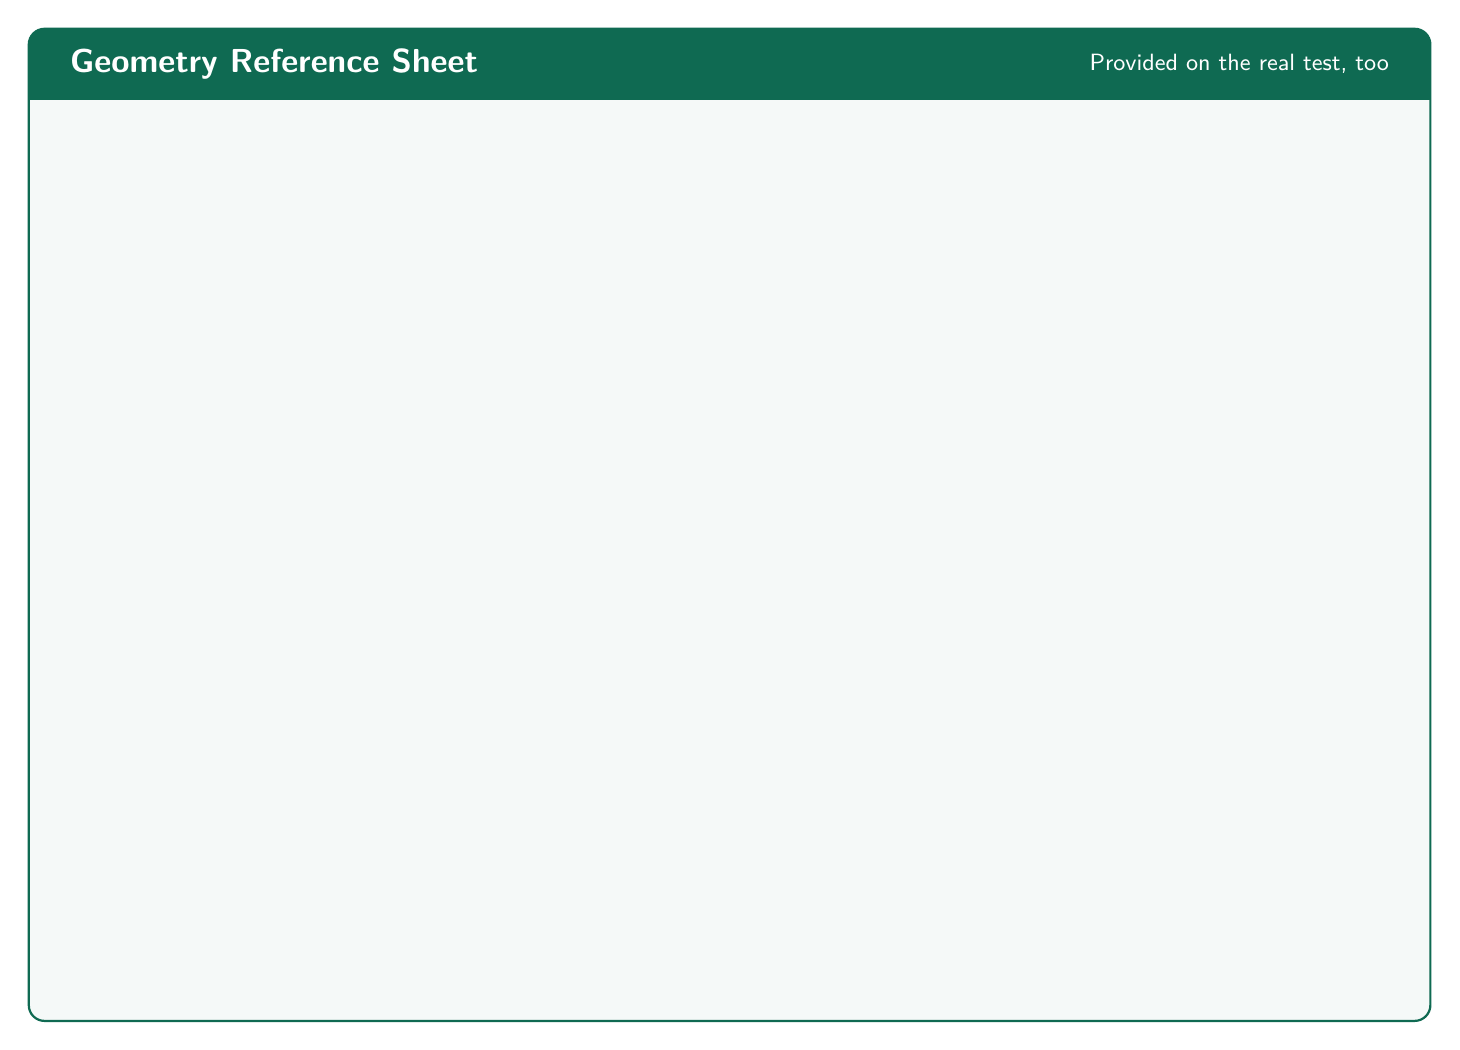
\begin{tikzpicture}
\draw[accent,line width=0.8pt,rounded corners=2mm,fill=badge!12] (0,0) rectangle (178mm,-126mm);
\fill[accent,rounded corners=2mm] (0,0) rectangle (178mm,-9mm);
\fill[accent] (0,-5mm) rectangle (178mm,-9mm);
\node[anchor=west,text=white,font=\sffamily\bfseries\fontsize{12}{14}\selectfont] at (4mm,-4.5mm) {Geometry Reference Sheet};
\node[anchor=east,text=white,font=\sffamily\fontsize{8.5}{10}\selectfont] at (174mm,-4.5mm) {Provided on the real test, too};
\end{tikzpicture}
\end{textblock*}

\newcommand{\refcell}[3]{\begin{textblock*}{42mm}(#1mm,#2mm)\begin{minipage}[t][36mm][t]{42mm}\centering #3\end{minipage}\end{textblock*}}
\newcommand{\refin}[2]{\parbox[b][26mm][b]{42mm}{\centering #1}\par\vspace{1.6mm}{\fontsize{9.6}{11.5}\selectfont #2}}
\tikzset{rf/.style={ink,line width=0.65pt},lb/.style={font=\fontsize{8.5}{9.5}\selectfont,inner sep=1.2pt}}

% ---------- row 1
\refcell{18}{167}{\refin{\begin{tikzpicture}[scale=1.25]
\draw[rf] (0,0) circle (9mm); \draw[rf] (0,0)--(9mm,0); \fill[ink] (0,0) circle (0.7pt);
\node[lb,above] at (4.5mm,0) {$r$};
\end{tikzpicture}}{Circle\\$A=\pi r^{2}$,\; $C=2\pi r$}}
\refcell{62}{167}{\refin{\begin{tikzpicture}[scale=1.25]
\draw[rf] (0,0) rectangle (22mm,12mm);
\node[lb,below] at (11mm,0) {$\ell$}; \node[lb,right] at (22mm,6mm) {$w$};
\end{tikzpicture}}{Rectangle\\$A=\ell w$}}
\refcell{106}{167}{\refin{\begin{tikzpicture}[scale=1.25]
\draw[rf] (0,0)--(22mm,0)--(7mm,13mm)--cycle;
\draw[rf,dashed] (7mm,0)--(7mm,13mm);
\draw[rf] (7mm,0)++(0,1.8mm)--++(1.8mm,0)--++(0,-1.8mm);
\node[lb,below] at (11mm,0) {$b$}; \node[lb,left] at (7mm,6.5mm) {$h$};
\end{tikzpicture}}{Triangle\\$A=\tfrac12 bh$}}
\refcell{150}{167}{\refin{\begin{tikzpicture}[scale=1.25]
\draw[rf] (0,0)--(18mm,0)--(0,12mm)--cycle;
\draw[rf] (0,1.8mm)--(1.8mm,1.8mm)--(1.8mm,0);
\node[lb,below] at (9mm,0) {$a$}; \node[lb,left] at (0,6mm) {$b$}; \node[lb,above right] at (9mm,6mm) {$c$};
\end{tikzpicture}}{Right triangle\\$c^{2}=a^{2}+b^{2}$}}

% ---------- row 2
\refcell{18}{204}{\refin{\begin{tikzpicture}[scale=1.25]
\draw[rf] (0,0)--(19.053mm,0)--(0,11mm)--cycle;
\draw[rf] (0,1.8mm)--(1.8mm,1.8mm)--(1.8mm,0);
\node[lb,below] at (9.5mm,0) {$x\sqrt3$}; \node[lb,left] at (0,5.5mm) {$x$}; \node[lb,above right] at (9.5mm,5.5mm) {$2x$};
\node[lb] at (14.6mm,1.9mm) {\fontsize{6.5}{7}\selectfont$30^\circ$}; \node[lb] at (3.2mm,8.2mm) {\fontsize{6.5}{7}\selectfont$60^\circ$};
\end{tikzpicture}}{$30^\circ$--$60^\circ$--$90^\circ$ triangle}}
\refcell{62}{204}{\refin{\begin{tikzpicture}[scale=1.25]
\draw[rf] (0,0)--(10mm,0)--(0,10mm)--cycle;
\draw[rf] (0,1.8mm)--(1.8mm,1.8mm)--(1.8mm,0);
\node[lb,below] at (5mm,0) {$s$}; \node[lb,left] at (0,5mm) {$s$}; \node[lb,above right] at (5mm,5mm) {$s\sqrt2$};
\end{tikzpicture}}{$45^\circ$--$45^\circ$--$90^\circ$ triangle}}
\refcell{106}{204}{\refin{\begin{tikzpicture}[scale=1.2]
\draw[rf] (0,0) rectangle (16mm,9mm);
\draw[rf] (16mm,9mm)--(22mm,13mm)--(6mm,13mm)--(0,9mm);
\draw[rf] (16mm,0)--(22mm,4mm)--(22mm,13mm);
\draw[rf,dashed] (6mm,13mm)--(6mm,4mm)--(22mm,4mm); \draw[rf,dashed] (0,0)--(6mm,4mm);
\node[lb,below] at (8mm,0) {$\ell$}; \node[lb,right] at (22mm,8.5mm) {$h$}; \node[lb,below right] at (19mm,2mm) {$w$};
\end{tikzpicture}}{Rectangular solid\\$V=\ell wh$}}
\refcell{150}{204}{\refin{\begin{tikzpicture}[scale=1.2]
\draw[rf] (0,2.2mm) ellipse (7mm and 2.2mm);
\draw[rf] (-7mm,2.2mm)--(-7mm,14mm); \draw[rf] (7mm,2.2mm)--(7mm,14mm);
\draw[rf] (0,14mm) ellipse (7mm and 2.2mm);
\draw[rf,dashed] (0,14mm)--(7mm,14mm); \fill[ink] (0,14mm) circle (0.6pt);
\node[lb,above] at (3.5mm,14mm) {$r$}; \node[lb,right] at (7mm,8mm) {$h$};
\end{tikzpicture}}{Right circular cylinder\\$V=\pi r^{2}h$}}

% ---------- row 3
\refcell{18}{241}{\refin{\begin{tikzpicture}[scale=1.15]
\draw[rf] (0,0) circle (10mm);
\draw[rf] (-10mm,0) arc (180:360:10mm and 2.8mm); \draw[rf,dashed] (-10mm,0) arc (180:0:10mm and 2.8mm);
\draw[rf] (0,0)--(10mm,0); \fill[ink] (0,0) circle (0.7pt); \node[lb,above] at (5mm,0) {$r$};
\end{tikzpicture}}{Sphere\\$V=\tfrac43\pi r^{3}$}}
\refcell{62}{241}{\refin{\begin{tikzpicture}[scale=1.2]
\draw[rf] (0,2.2mm) ellipse (7mm and 2.2mm);
\draw[rf] (-7mm,2.2mm)--(0,16mm)--(7mm,2.2mm);
\draw[rf,dashed] (0,16mm)--(0,2.2mm); \draw[rf,dashed] (0,2.2mm)--(7mm,2.2mm);
\fill[ink] (0,2.2mm) circle (0.6pt);
\node[lb,left] at (0,9.5mm) {$h$}; \node[lb,above] at (3.5mm,2.2mm) {$r$};
\end{tikzpicture}}{Right circular cone\\$V=\tfrac13\pi r^{2}h$}}
\refcell{106}{241}{\refin{\begin{tikzpicture}[scale=1.2]
\draw[rf] (0,0)--(16mm,0)--(22mm,4mm); \draw[rf] (0,0)--(10mm,15mm)--(16mm,0); \draw[rf] (10mm,15mm)--(22mm,4mm);
\draw[rf,dashed] (0,0)--(6mm,4mm)--(22mm,4mm); \draw[rf,dashed] (6mm,4mm)--(10mm,15mm);
\node[lb,below] at (8mm,0) {$\ell$}; \node[lb,below right] at (19mm,2mm) {$w$}; \node[lb,left] at (10mm,9.5mm) {$h$};
\end{tikzpicture}}{Rectangular pyramid\\$V=\tfrac13\ell wh$}}
\begin{textblock*}{40mm}(151mm,247mm)
{\fontsize{9.2}{12}\selectfont\raggedright
\textcolor{accent}{\rule[0.3mm]{1.6mm}{1.6mm}}\; A circle has 360 degrees of arc.\par\vspace{1.2mm}
\textcolor{accent}{\rule[0.3mm]{1.6mm}{1.6mm}}\; The angles of a triangle add up to 180 degrees.\par\vspace{1.2mm}
\textcolor{accent}{\rule[0.3mm]{1.6mm}{1.6mm}}\; $r$ radius, $\ell$ length, $w$ width, $b$ base, $h$ height.\par}
\end{textblock*}

\clearpage

% ===== Module 1, page 1 =====
\topicheader{5}{Mock Test 5}
\pagefooter{2}
\colrule{34}{236}
\mbox{}%
\pagekicker{Mock 5 \textperiodcentered{} Module 1 \textperiodcentered{} 22 questions \textperiodcentered{} 35 minutes}{Questions 1--8}
\begin{textblock*}{\COLW}(\LCOL,34mm)
{\fontsize{10.4}{13.4}\selectfont
\parbox[t][233mm][t]{\COLW}{%
\noindent\pnum{1} If $11-2x=-7$, what is the value of $x$?\par\vspace{2.2mm}
\hspace*{7mm}(A)\ $2$\\[1.8mm]
\hspace*{7mm}(B)\ $9$\\[1.8mm]
\hspace*{7mm}(C)\ $18$\\[1.8mm]
\hspace*{7mm}(D)\ $-9$
\vfill

\noindent\pnum{2} Which of the following is equivalent to $3x(x-4)+5x$?\par\vspace{2.2mm}
\hspace*{7mm}(A)\ $3x^2-17x$\\[1.8mm]
\hspace*{7mm}(B)\ $3x^2-12x+5$\\[1.8mm]
\hspace*{7mm}(C)\ $3x^2-7$\\[1.8mm]
\hspace*{7mm}(D)\ $3x^2-7x$
\vfill

\noindent\pnum{3} A landscaping crew has spread mulch over 35\% of a lawn that has an area of 240 square meters. What area, in square meters, has been covered with mulch?\gridbox
\vfill

\noindent\pnum{4} In an isosceles triangle, each of the two base angles measures $54^{\circ}$. What is the measure, in degrees, of the vertex angle?\par\vspace{2.2mm}
\hspace*{7mm}(A)\ $72$\\[1.8mm]
\hspace*{7mm}(B)\ $54$\\[1.8mm]
\hspace*{7mm}(C)\ $108$\\[1.8mm]
\hspace*{7mm}(D)\ $126$
\vfill}}
\end{textblock*}
\begin{textblock*}{\COLW}(\RCOL,34mm)
{\fontsize{10.4}{13.4}\selectfont
\parbox[t][233mm][t]{\COLW}{%
\noindent\pnum{5} If $3(x+2)=2(x+7)$, what is the value of $x$?\par\vspace{2.2mm}
\hspace*{7mm}(A)\ $-20$\\[1.8mm]
\hspace*{7mm}(B)\ $1$\\[1.8mm]
\hspace*{7mm}(C)\ $8$\\[1.8mm]
\hspace*{7mm}(D)\ $12$
\vfill

\noindent\pnum{6} Which of the following is a zero of the polynomial $p(x)=(x-3)(x+5)(2x-1)$?\par\vspace{2.2mm}
\hspace*{7mm}(A)\ $-3$\\[1.8mm]
\hspace*{7mm}(B)\ $2$\\[1.8mm]
\hspace*{7mm}(C)\ $5$\\[1.8mm]
\hspace*{7mm}(D)\ $\dfrac{1}{2}$
\vfill

\noindent\pnum{7} The student council needs to raise at least \$450 by selling pennants for \$6 each. What is the least number of pennants it must sell?\gridbox
\vfill

\noindent\pnum{8} In the $xy$-plane, the graph of $y=(x-2)(x+6)$ crosses the $y$-axis at the point $(0,k)$. What is the value of $k$?\par\vspace{2.2mm}
\hspace*{7mm}(A)\ $-4$\\[1.8mm]
\hspace*{7mm}(B)\ $-12$\\[1.8mm]
\hspace*{7mm}(C)\ $4$\\[1.8mm]
\hspace*{7mm}(D)\ $12$
\vfill}}
\end{textblock*}
\clearpage

% ===== Module 1, page 2 =====
\topicheader{5}{Mock Test 5}
\pagefooter{3}
\colrule{34}{236}
\mbox{}%
\pagekicker{Mock 5 \textperiodcentered{} Module 1 \textperiodcentered{} 22 questions \textperiodcentered{} 35 minutes}{Questions 9--16}
\begin{textblock*}{\COLW}(\LCOL,34mm)
{\fontsize{10.4}{13.4}\selectfont
\parbox[t][233mm][t]{\COLW}{%
\noindent\pnum{9} The table shows two data sets, $P$ and $Q$, each with five values. Which of the following statements is true?\figwrap{\begin{tabular}{|l|c|c|c|c|c|}
\hline
Set $P$ & 12 & 14 & 16 & 18 & 20\\\hline
Set $Q$ & 14 & 15 & 16 & 17 & 18\\\hline
\end{tabular}}\par\vspace{2.2mm}
\hspace*{7mm}(A)\ The two sets have the same mean, and Set $P$ has the greater standard deviation.\\[1.8mm]
\hspace*{7mm}(B)\ The two sets have the same mean, and Set $Q$ has the greater standard deviation.\\[1.8mm]
\hspace*{7mm}(C)\ Set $P$ has the greater mean, and Set $P$ has the greater standard deviation.\\[1.8mm]
\hspace*{7mm}(D)\ The two sets have the same mean and the same standard deviation.
\vfill

\noindent\pnum{10} A robotics club has a budget of \$900. It buys 10 kits at \$45 each and will spend part of the remaining budget on battery packs that cost \$12 each. What is the greatest number of battery packs the club can buy without going over its budget?\par\vspace{2.2mm}
\hspace*{7mm}(A)\ $20$\\[1.8mm]
\hspace*{7mm}(B)\ $36$\\[1.8mm]
\hspace*{7mm}(C)\ $37$\\[1.8mm]
\hspace*{7mm}(D)\ $38$
\vfill

\noindent\pnum{11} A garden center sells soil by the bag and mulch by the bag. Three bags of soil and two bags of mulch cost \$38. Five bags of soil and four bags of mulch cost \$68. What is the cost, in dollars, of one bag of soil?\gridbox
\vfill

\noindent\pnum{12} What is the remainder when $p(x)=2x^3-5x^2+x-4$ is divided by $x-2$?\par\vspace{2.2mm}
\hspace*{7mm}(A)\ $-42$\\[1.8mm]
\hspace*{7mm}(B)\ $-6$\\[1.8mm]
\hspace*{7mm}(C)\ $-4$\\[1.8mm]
\hspace*{7mm}(D)\ $6$
\vfill}}
\end{textblock*}
\begin{textblock*}{\COLW}(\RCOL,34mm)
{\fontsize{10.4}{13.4}\selectfont
\parbox[t][233mm][t]{\COLW}{%
\noindent\pnum{13} A landscaper spreads mulch 7 centimeters deep over a rectangular flower bed that is 3 meters long and 2 meters wide. Mulch is sold in bags that each hold 40 liters. What is the least number of bags needed to cover the bed? (1 cubic meter $=$ 1,000 liters.)\par\vspace{2.2mm}
\hspace*{7mm}(A)\ $11$\\[1.8mm]
\hspace*{7mm}(B)\ $2$\\[1.8mm]
\hspace*{7mm}(C)\ $10$\\[1.8mm]
\hspace*{7mm}(D)\ $105$
\vfill

\noindent\pnum{14} A steel supplier raised its price per tonne by 20\%. A month later it lowered the new price by 20\%, to \$720 per tonne. What was the price per tonne, in dollars, before the increase?\gridbox
\vfill

\noindent\pnum{15} The annual energy output, in kilowatt-hours (kWh), of a solar panel is modeled by $E(t)=5400(0.992)^{t}$, where $t$ is the number of years after the panel was installed. Which of the following is the best interpretation of the number $0.992$ in this context?\par\vspace{2.2mm}
\hspace*{7mm}(A)\ The panel's output decreases by 0.992\% each year.\\[1.8mm]
\hspace*{7mm}(B)\ The panel's output decreases by 99.2\% each year.\\[1.8mm]
\hspace*{7mm}(C)\ The panel's output decreases by 43.2 kWh each year.\\[1.8mm]
\hspace*{7mm}(D)\ The panel's output decreases by 0.8\% each year.
\vfill

\noindent\pnum{16} In the $xy$-plane, line $\ell$ is parallel to the graph of $3x+4y=20$ and passes through the point $(4,1)$. What is the $y$-intercept of line $\ell$?\par\vspace{2.2mm}
\hspace*{7mm}(A)\ $-2$\\[1.8mm]
\hspace*{7mm}(B)\ $3$\\[1.8mm]
\hspace*{7mm}(C)\ $4$\\[1.8mm]
\hspace*{7mm}(D)\ $16$
\vfill}}
\end{textblock*}
\clearpage

% ===== Module 1, page 3 =====
\topicheader{5}{Mock Test 5}
\pagefooter{4}
\colrule{34}{236}
\mbox{}%
\pagekicker{Mock 5 \textperiodcentered{} Module 1 \textperiodcentered{} 22 questions \textperiodcentered{} 35 minutes}{Questions 17--22}
\begin{textblock*}{\COLW}(\LCOL,34mm)
{\fontsize{10.4}{13.4}\selectfont
\parbox[t][233mm][t]{\COLW}{%
\noindent\pnum{17} The sum of three consecutive odd integers is less than 90. What is the greatest possible value of the smallest of the three integers?\par\vspace{2.2mm}
\hspace*{7mm}(A)\ $25$\\[1.8mm]
\hspace*{7mm}(B)\ $27$\\[1.8mm]
\hspace*{7mm}(C)\ $28$\\[1.8mm]
\hspace*{7mm}(D)\ $29$
\vfill

\noindent\pnum{18} The expression $(3x+2)^2-(3x-2)^2$ is equivalent to $kx$, where $k$ is a constant. What is the value of $k$?\gridbox
\vfill

\noindent\pnum{19} Which of the following quadratic equations has the solutions $x=-\dfrac{3}{2}$ and $x=4$?\par\vspace{2.2mm}
\hspace*{7mm}(A)\ $2x^2-5x-12=0$\\[1.8mm]
\hspace*{7mm}(B)\ $2x^2+5x-12=0$\\[1.8mm]
\hspace*{7mm}(C)\ $2x^2-11x+12=0$\\[1.8mm]
\hspace*{7mm}(D)\ $2x^2+2x-12=0$
\vfill}}
\end{textblock*}
\begin{textblock*}{\COLW}(\RCOL,34mm)
{\fontsize{10.4}{13.4}\selectfont
\parbox[t][233mm][t]{\COLW}{%
\noindent\pnum{20} The function $f$ is defined by $f(x)=-2(x-3)^2+18$. For how many integer values of $x$ is $f(x)$ positive?\par\vspace{2.2mm}
\hspace*{7mm}(A)\ $3$\\[1.8mm]
\hspace*{7mm}(B)\ $6$\\[1.8mm]
\hspace*{7mm}(C)\ $7$\\[1.8mm]
\hspace*{7mm}(D)\ $5$
\vfill

\noindent\pnum{21} A right circular cone has a height of 12 centimeters and a base radius of 9 centimeters. A plane parallel to the base cuts off a smaller cone at the top, and the smaller cone has a height of 4 centimeters. The volume of the remaining solid, between the base and the cutting plane, is $k\pi$ cubic centimeters. What is the value of $k$?\gridbox
\vfill

\noindent\pnum{22} Two hikers start at opposite ends of a 27-kilometer trail at the same time and walk toward each other at constant speeds. One hiker walks 1.5 kilometers per hour faster than the other, and they meet after exactly 3 hours. After they meet, how many minutes does it take the slower hiker to reach the far end of the trail?\par\vspace{2.2mm}
\hspace*{7mm}(A)\ $129$\\[1.8mm]
\hspace*{7mm}(B)\ $180$\\[1.8mm]
\hspace*{7mm}(C)\ $252$\\[1.8mm]
\hspace*{7mm}(D)\ $315$
\vfill}}
\end{textblock*}
\clearpage

% ===== Module 2, page 1 =====
\topicheader{5}{Mock Test 5}
\pagefooter{5}
\colrule{34}{236}
\mbox{}%
\pagekicker{Mock 5 \textperiodcentered{} Module 2 \textperiodcentered{} 22 questions \textperiodcentered{} 35 minutes}{Questions 1--8}
\begin{textblock*}{\COLW}(\LCOL,34mm)
{\fontsize{10.4}{13.4}\selectfont
\parbox[t][233mm][t]{\COLW}{%
\noindent\pnum{1} If $5x-3=2x+18$, what is the value of $x$?\par\vspace{2.2mm}
\hspace*{7mm}(A)\ $5$\\[1.8mm]
\hspace*{7mm}(B)\ $\dfrac{15}{7}$\\[1.8mm]
\hspace*{7mm}(C)\ $7$\\[1.8mm]
\hspace*{7mm}(D)\ $21$
\vfill

\noindent\pnum{2} The function $f$ is defined by $f(x)=x^2-4x+1$. What is the value of $f(3)$?\par\vspace{2.2mm}
\hspace*{7mm}(A)\ $-2$\\[1.8mm]
\hspace*{7mm}(B)\ $-4$\\[1.8mm]
\hspace*{7mm}(C)\ $-20$\\[1.8mm]
\hspace*{7mm}(D)\ $22$
\vfill

\noindent\pnum{3} A driver completed a 300-mile trip. She drove the first 120 miles at a constant speed of 60 miles per hour and the remaining 180 miles at a constant speed of 45 miles per hour. What was her average speed, in miles per hour, for the entire trip?\par\vspace{2.2mm}
\hspace*{7mm}(A)\ $45$\\[1.8mm]
\hspace*{7mm}(B)\ $52.5$\\[1.8mm]
\hspace*{7mm}(C)\ $105$\\[1.8mm]
\hspace*{7mm}(D)\ $50$
\vfill

\noindent\pnum{4} In the $xy$-plane, the graph of $kx+6y=30$, where $k$ is a constant, is parallel to the graph of $2x+3y=7$. What is the $x$-coordinate of the point where the graph of $kx+6y=30$ crosses the $x$-axis?\gridbox
\vfill}}
\end{textblock*}
\begin{textblock*}{\COLW}(\RCOL,34mm)
{\fontsize{10.4}{13.4}\selectfont
\parbox[t][233mm][t]{\COLW}{%
\noindent\pnum{5} The polynomial $p(x)$ has degree 2, and its zeros are $x=-3$ and $x=\frac12$. The graph of $y=p(x)$ crosses the $y$-axis at the point $(0,-9)$. Which of the following could be $p(x)$?\par\vspace{2.2mm}
\hspace*{7mm}(A)\ $2x^2+5x-3$\\[1.8mm]
\hspace*{7mm}(B)\ $6x^2+15x-9$\\[1.8mm]
\hspace*{7mm}(C)\ $6x^2-15x-9$\\[1.8mm]
\hspace*{7mm}(D)\ $6x^2+15x+9$
\vfill

\noindent\pnum{6} A solid right circular cylinder has a volume of $200\pi$ cubic centimeters and a height of 8 centimeters. What is the total surface area, in square centimeters, of the cylinder, including both circular bases?\par\vspace{2.2mm}
\hspace*{7mm}(A)\ $80\pi$\\[1.8mm]
\hspace*{7mm}(B)\ $105\pi$\\[1.8mm]
\hspace*{7mm}(C)\ $130\pi$\\[1.8mm]
\hspace*{7mm}(D)\ $200\pi$
\vfill

\noindent\pnum{7} A gardener is planting a rectangular bed that has an area of 12 square meters. Each tomato plant needs 0.6 square meter and each pepper plant needs 0.4 square meter. The gardener will plant $x$ tomato plants and $y$ pepper plants, using no more than the available space, and wants at least twice as many pepper plants as tomato plants. Which of the following systems of inequalities represents these conditions?\par\vspace{2.2mm}
\hspace*{7mm}(A)\ $0.4x+0.6y\le12$ and $y\ge2x$\\[1.8mm]
\hspace*{7mm}(B)\ $0.6x+0.4y\ge12$ and $y\ge2x$\\[1.8mm]
\hspace*{7mm}(C)\ $0.6x+0.4y\le12$ and $x\ge2y$\\[1.8mm]
\hspace*{7mm}(D)\ $0.6x+0.4y\le12$ and $y\ge2x$
\vfill

\noindent\pnum{8} If $2^{x+1}\cdot4^{x-2}=64$, what is the value of $x$?\gridbox
\vfill}}
\end{textblock*}
\clearpage

% ===== Module 2, page 2 =====
\topicheader{5}{Mock Test 5}
\pagefooter{6}
\colrule{34}{236}
\mbox{}%
\pagekicker{Mock 5 \textperiodcentered{} Module 2 \textperiodcentered{} 22 questions \textperiodcentered{} 35 minutes}{Questions 9--15}
\begin{textblock*}{\COLW}(\LCOL,34mm)
{\fontsize{10.4}{13.4}\selectfont
\parbox[t][233mm][t]{\COLW}{%
\noindent\pnum{9} A data set of 12 values has a mean of 50 and a standard deviation of 8. A 13th value, equal to 50, is added to the data set. Which of the following must be true of the new data set of 13 values?\par\vspace{2.2mm}
\hspace*{7mm}(A)\ The mean is 50, and the standard deviation is less than 8.\\[1.8mm]
\hspace*{7mm}(B)\ The mean is 50, and the standard deviation is exactly 8.\\[1.8mm]
\hspace*{7mm}(C)\ The mean is 50, and the standard deviation is greater than 8.\\[1.8mm]
\hspace*{7mm}(D)\ The mean is less than 50, and the standard deviation is less than 8.
\vfill

\noindent\pnum{10} In the system below, $k$ is a constant. If the system has infinitely many solutions, what is the value of $k$?\dsp{$y=2x+7$}\dsp{$4x-2y=k$}\par\vspace{2.2mm}
\hspace*{7mm}(A)\ $-7$\\[1.8mm]
\hspace*{7mm}(B)\ $-14$\\[1.8mm]
\hspace*{7mm}(C)\ $7$\\[1.8mm]
\hspace*{7mm}(D)\ $14$
\vfill

\noindent\pnum{11} The point $(4,9)$ lies on the graph of $y=f(x)$ in the $xy$-plane. The function $g$ is defined by $g(x)=2f(x-1)-5$. The point $(a,b)$ lies on the graph of $y=g(x)$ and corresponds to the point $(4,9)$ on the graph of $f$. What is the value of $a+b$?\gridbox
\vfill

\noindent\pnum{12} How many integers $x$ satisfy both $3x-7>8$ and $2x+5\le31$?\par\vspace{2.2mm}
\hspace*{7mm}(A)\ $7$\\[1.8mm]
\hspace*{7mm}(B)\ $9$\\[1.8mm]
\hspace*{7mm}(C)\ $8$\\[1.8mm]
\hspace*{7mm}(D)\ $13$
\vfill}}
\end{textblock*}
\begin{textblock*}{\COLW}(\RCOL,34mm)
{\fontsize{10.4}{13.4}\selectfont
\parbox[t][233mm][t]{\COLW}{%
\noindent\pnum{13} A shipping company charges \$9 for the first kilogram of a package and a fixed amount for each additional kilogram or fraction of a kilogram. A package weighing 6.5 kilograms costs \$39 to ship. How much would it cost, in dollars, to ship a package weighing 12.2 kilograms?\par\vspace{2.2mm}
\hspace*{7mm}(A)\ $69$\\[1.8mm]
\hspace*{7mm}(B)\ $64$\\[1.8mm]
\hspace*{7mm}(C)\ $65$\\[1.8mm]
\hspace*{7mm}(D)\ $70$
\vfill

\noindent\pnum{14} A triangular garden plot $ABC$ has sides $AB=13$ meters, $BC=14$ meters, and $CA=15$ meters. A circular pond inside the plot is tangent to all three sides and touches side $\overline{BC}$ at point $P$. Point $P$ divides $\overline{BC}$ into two parts. What is the length, in meters, of the longer part?\figwrap{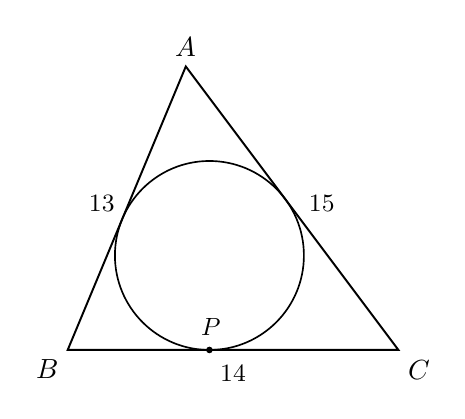
\begin{tikzpicture}[scale=0.3]
\coordinate (B) at (0,0); \coordinate (C) at (14,0); \coordinate (A) at (5,12);
\draw[line width=0.7pt] (A)--(B)--(C)--cycle;
\draw[line width=0.6pt] (6,4) circle (4);
\fill (6,0) circle (0.14);
\node[below left] at (B) {$B$}; \node[below right] at (C) {$C$}; \node[above] at (A) {$A$};
\node[above,font=\small] at (6,0.2) {$P$};
\node[left,font=\small] at (2.4,6.2) {13}; \node[right,font=\small] at (9.8,6.2) {15};
\node[below,font=\small] at (7,-0.2) {14};
\end{tikzpicture}}\par\vspace{2.2mm}
\hspace*{7mm}(A)\ $6$\\[1.8mm]
\hspace*{7mm}(B)\ $7$\\[1.8mm]
\hspace*{7mm}(C)\ $9$\\[1.8mm]
\hspace*{7mm}(D)\ $8$
\vfill

\noindent\pnum{15} For a real number $x$, $\sqrt{x+7}+\sqrt{x-1}=4$. What is the value of $\sqrt{x+7}-\sqrt{x-1}$?\gridbox
\vfill}}
\end{textblock*}
\clearpage

% ===== Module 2, page 3 =====
\topicheader{5}{Mock Test 5}
\pagefooter{7}
\colrule{34}{236}
\mbox{}%
\pagekicker{Mock 5 \textperiodcentered{} Module 2 \textperiodcentered{} 22 questions \textperiodcentered{} 35 minutes}{Questions 16--22}
\begin{textblock*}{\COLW}(\LCOL,34mm)
{\fontsize{10.4}{13.4}\selectfont
\parbox[t][233mm][t]{\COLW}{%
\noindent\pnum{16} At a school with 240 students, 150 students are in the band, 110 students are in the chorus, and 40 students are in neither. One student is selected at random from only those students who are in exactly one of the two groups. What is the probability that the selected student is in the band?\par\vspace{2.2mm}
\hspace*{7mm}(A)\ $\dfrac{3}{5}$\\[1.8mm]
\hspace*{7mm}(B)\ $\dfrac{9}{14}$\\[1.8mm]
\hspace*{7mm}(C)\ $\dfrac{15}{26}$\\[1.8mm]
\hspace*{7mm}(D)\ $\dfrac{5}{8}$
\vfill

\noindent\pnum{17} A rectangular garden bed has an area of 11 square meters, and its length is 6 meters more than its width. What is the perimeter, in meters, of the bed?\par\vspace{2.2mm}
\hspace*{7mm}(A)\ $4\sqrt{5}$\\[1.8mm]
\hspace*{7mm}(B)\ $2\sqrt{47}$\\[1.8mm]
\hspace*{7mm}(C)\ $8\sqrt{5}$\\[1.8mm]
\hspace*{7mm}(D)\ $24$
\vfill

\noindent\pnum{18} In the $xy$-plane, a line with a positive $x$-intercept and a positive $y$-intercept passes through the point $(6,4)$. The $x$-intercept is twice the $y$-intercept. What is the area, in square units, of the triangle formed by this line and the two axes?\gridbox
\vfill

\noindent\pnum{19} What is the sum of the $y$-coordinates of all points of intersection of the graphs of $y=x^2-3$ and $x^2+y^2=9$ in the $xy$-plane?\par\vspace{2.2mm}
\hspace*{7mm}(A)\ $1$\\[1.8mm]
\hspace*{7mm}(B)\ $-1$\\[1.8mm]
\hspace*{7mm}(C)\ $4$\\[1.8mm]
\hspace*{7mm}(D)\ $7$
\vfill}}
\end{textblock*}
\begin{textblock*}{\COLW}(\RCOL,34mm)
{\fontsize{10.4}{13.4}\selectfont
\parbox[t][233mm][t]{\COLW}{%
\noindent\pnum{20} Positions along a straight highway are measured in kilometers from a town. A service station is at position $-1$ and a rest area is at position $3$. A cyclist at position $x$ is exactly twice as far from the rest area as from the service station. What is the sum of all possible values of $x$?\par\vspace{2.2mm}
\hspace*{7mm}(A)\ $-5$\\[1.8mm]
\hspace*{7mm}(B)\ $-\dfrac{5}{3}$\\[1.8mm]
\hspace*{7mm}(C)\ $\dfrac{1}{3}$\\[1.8mm]
\hspace*{7mm}(D)\ $-\dfrac{14}{3}$
\vfill

\noindent\pnum{21} A circular steel disc has a radius of 25 centimeters. Two parallel straight cuts are made across the disc, one 14 centimeters long and the other 40 centimeters long, with the center of the disc between the two cuts. What is the distance, in centimeters, between the two cuts?\figwrap{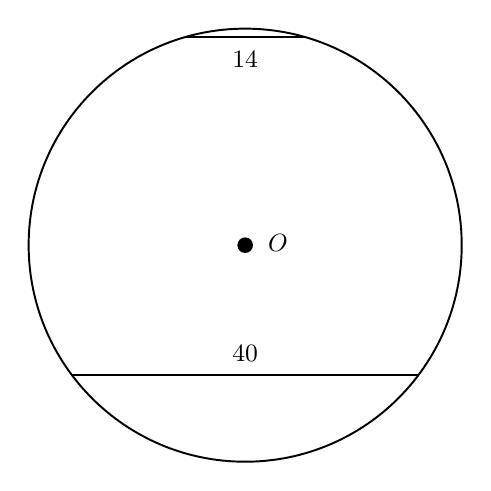
\begin{tikzpicture}[scale=0.11]
\draw[line width=0.7pt] (0,0) circle (25);
\draw[line width=0.7pt] (-7,24)--(7,24);
\draw[line width=0.7pt] (-20,-15)--(20,-15);
\fill (0,0) circle (0.9);
\node[right,font=\small] at (1.6,0.2) {$O$};
\node[below,font=\small] at (0,23.6) {14};
\node[above,font=\small] at (0,-14.6) {40};
\end{tikzpicture}}\gridbox
\vfill

\noindent\pnum{22} When the polynomial $p(x)$ is divided by $x-2$, the remainder is 5. When $p(x)$ is divided by $x+3$, the remainder is $-15$. When $p(x)$ is divided by $x^2+x-6$, the remainder is $ax+b$, where $a$ and $b$ are constants. What is the value of $b$?\par\vspace{2.2mm}
\hspace*{7mm}(A)\ $-15$\\[1.8mm]
\hspace*{7mm}(B)\ $-3$\\[1.8mm]
\hspace*{7mm}(C)\ $4$\\[1.8mm]
\hspace*{7mm}(D)\ $5$
\vfill}}
\end{textblock*}
\clearpage

\end{document}
